\section{PHƯƠNG TRÌNH, BẤT PHƯƠNG TRÌNH MŨ VÀ LOGARIT}
\subsection{LÝ THUYẾT CẦN NHỚ}
\subsubsection{Công thức nghiệm của phương trình mũ}
\begin{itemize}
\item [\faCheckSquareO]Dạng \fbox{$a^x=b$} (1), với $a>0$ và $a \ne 1$.
	\item [\faCheckSquareO] Về mặt đồ thị, nghiệm của (1) là hoành độ giao điểm của đồ thị $y=a^x$ với đường thẳng $y=b$ (nằm ngang). 
	\immini{Từ hình vẽ, ta có các kết quả sau:
			\begin{listEX}[1]
				\item [\ding{172}] $b>0$ (1) có nghiệm duy nhất $x=\log_ab$.
				\item [\ding{173}] $b\le 0$ (1) vô nghiệm.
			\end{listEX}
		}{	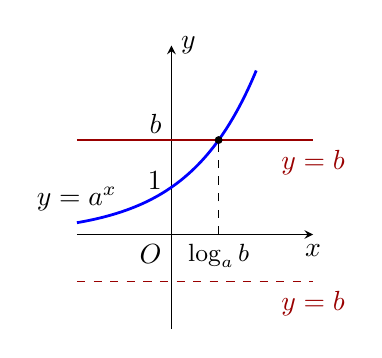
\begin{tikzpicture}[smooth,samples=300,scale=0.6,>=stealth]
		\draw[->] (-2,0)--(3,0) node[below]{$x$};
		\draw[->] (0,-2)--(0,4) node[right]{$y$};
		\draw (0,0) node[below left]{$O$};
		\draw[line width=1pt,color=blue,domain=-2:1.8] plot(\x,{2^(\x)});
		\draw[color=red!60!black,line width=1pt] (-2,2)--(3,2) node[below]{$y=b$};
		\draw[dashed,color=red!60!black] (-2,-1)--(3,-1) node[below]{$y=b$};
		\draw[dashed] (1,0)node[below]{\small$\log_ab$}--(1,2);
		\draw[fill=black](1,2) circle(2pt);
		\node[above] at (-2,0.3) {$y=a^x$};
		\node[left] at (0,2.35) {$b$};
		\node[left] at (0,1.15) {$1$};
		\end{tikzpicture}}
\begin{khung4}{GHI NHỚ}
	Với $a>0$ và $a \ne 1$, $b>0$, ta có các công thức sau đây: 
	\begin{listEX}[2]
		\item [\ding{172}] $a^{f(x)}=b \Leftrightarrow f(x)=\log_ab$
		\item [\ding{173}] $a^{f(x)}=a^{g(x)} \Leftrightarrow f(x)=g(x)$
	\end{listEX}
\end{khung4}
\end{itemize}
\subsubsection{Công thức nghiệm của phương trình lôgarit}
\begin{itemize}
\item [\faCheckSquareO]Dạng \fbox{$\log_ax=b$} (2), với $a>0$ và $a \ne 1$.
		\item [\faCheckSquareO]Về mặt đồ thị, nghiệm của (2) là hoành độ giao điểm của đồ thị $y=\log_ax$ với đường thẳng $y=b$ (nằm ngang). 
	\immini{	
		Từ hình vẽ, ta có các kết quả sau:
		\begin{listEX}[1]
				\item [\ding{172}] Với mọi $b$, (2) luôn có nghiệm duy nhất.
				\item [\ding{173}] $\log_ax=b \Leftrightarrow x=a^b$.
			\end{listEX}
		}{	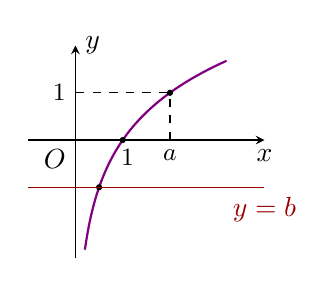
\begin{tikzpicture}[smooth,samples=300,scale=0.6,>=stealth]
			\draw[->] (-1,0)--(4,0) node[below]{$x$};
			\draw[->] (0,-2.5)--(0,2) node[right]{$y$};
			\draw (0,0) node[below left]{$O$};
			\draw[line width=0.8pt,color=violet,domain=0.2:3.2]plot(\x,{ln((\x))/ln(2)});
			\draw[fill=black] (1,0) circle(1.5pt) (2,1) circle(1.5pt) (0.5,-1) circle(1.5pt);
			\draw[dashed] (2,0)node[below]{\small$a$}--(2,1)--(0,1)node[left]{\small$1$};
			\draw[color=red!60!black] (-1,-1)--(4,-1) node[below]{$y=b$};
			\node[below] at (1.1,0) {\small$1$};
			\end{tikzpicture}}
		
\begin{khung4}{GHI NHỚ}
	Với $a>0$ và $a \ne 1$, $b$ bất kì, ta có các công thức sau đây: 
	\begin{listEX}[1]
		\item [\ding{172}] $\log_ax=b \Leftrightarrow x=a^b$.
		\item [\ding{173}] $\log_a{f(x)}=\log_a{g(x)}\Leftrightarrow \heva{&f(x)>0 \,(\text{ hoặc } g(x)>0)\\&f(x)=g(x)}$.
	\end{listEX}
\end{khung4}
\end{itemize}

\subsubsection{Công thức nghiệm của bất phương trình mũ}
Minh họa dạng \fbox{$a^x>b$}, với $a>0$ và $a \ne 1$.
\begin{center}
	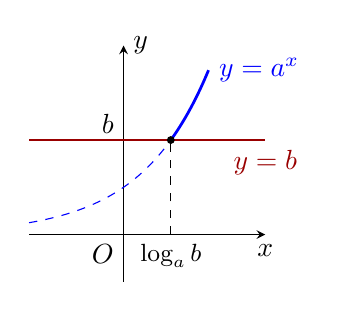
\begin{tikzpicture}[smooth,samples=300,scale=0.6,>=stealth]
		\draw[->] (-2,0)--(3,0) node[below]{$x$};
		\draw[->] (0,-1)--(0,4) node[right]{$y$};
		\draw (0,0) node[below left]{$O$};
		\draw[dashed,color=blue,domain=-2:1] plot(\x,{2^(\x)});
		\draw[line width=1pt,color=blue,domain=1:1.8] plot(\x,{2^(\x)})node[right]{$y=a^x$};
		\draw[color=red!60!black,line width=1pt] (-2,2)--(3,2) node[below]{$y=b$};
		\draw[dashed] (1,0)node[below]{\small$\log_ab$}--(1,2);
		\draw[fill=black](1,2) circle(2pt);
		\node[left] at (0,2.35) {$b$};
	\end{tikzpicture}
	\hspace{3cm}
	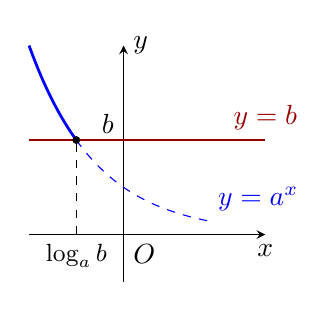
\begin{tikzpicture}[smooth,samples=300,scale=0.6,>=stealth]
		\draw[->] (-2,0)--(3,0) node[below]{$x$};
		\draw[->] (0,-1)--(0,4) node[right]{$y$};
		\draw (0,0) node[below right]{$O$};
		\draw[dashed,color=blue,domain=-1:1.8] plot(\x,{0.5^(\x)})node[above right]{$y=a^x$};
		\draw[line width=1pt,color=blue,domain=-2:-1] plot(\x,{0.5^(\x)});
		\draw[color=red!60!black,line width=1pt] (-2,2)--(3,2) node[above]{$y=b$};
		\draw[dashed] (-1,0)node[below]{\small$\log_ab$}--(-1,2);
		\draw[fill=black](-1,2) circle(2pt);
		\node[left] at (0,2.35) {$b$};
	\end{tikzpicture}
\end{center}
\begin{itemize}
	\item [$\bullet$] Nếu $b \le 0$ thì tập nghiệm của bất phương trình là $\mathbb{R}$.
	\item [$\bullet$] Nếu $b>0$, ta có hai trường hợp:
	\begin{tcolorbox}[colframe=cyan,colback=red!3!white,boxrule=0.5mm]
			\begin{listEX}[1]
			\item [\ding{172}] Với $a>1$ thì $a^x>b \Leftrightarrow x>\log_ab$ (Hình bên trái).
			\item [\ding{173}] Với $0<a<1$ thì $a^x>b \Leftrightarrow x<\log_ab$ (Hình bên phải).
		\end{listEX}
	\end{tcolorbox}
\end{itemize}
\subsubsection{Công thức nghiệm của bất phương trình lôgarit}
Minh họa dạng \fbox{$\log_ax>b$}, với $a>0$ và $a \ne 1$.
\begin{center}
	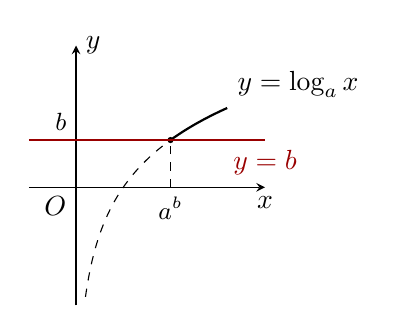
\begin{tikzpicture}[smooth,samples=300,scale=0.6,>=stealth]
		\draw[->] (-1,0)--(4,0) node[below]{$x$};
		\draw[->] (0,-2.5)--(0,3) node[right]{$y$};
		\draw (0,0) node[below left]{$O$};
		\draw[dashed,black,domain=0.2:2]plot(\x,{ln((\x))/ln(2)});
		\draw[line width=0.8pt,black,domain=2:3.2]plot(\x,{ln((\x))/ln(2)})node[above right]{$y=\log_ax$};
		\draw[fill=black] (2,1) circle(1.5pt);
		\draw[dashed] (2,0)node[below]{\small$a^b$}--(2,1)--(0,1)node[above left]{\small$b$};
		\draw[color=red!60!black,thick] (-1,1)--(4,1) node[below]{$y=b$};
	\end{tikzpicture}
	\hspace{3cm}
	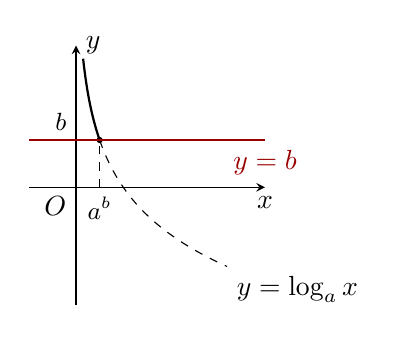
\begin{tikzpicture}[smooth,samples=300,scale=0.6,>=stealth]
		\draw[->] (-1,0)--(4,0) node[below]{$x$};
		\draw[->] (0,-2.5)--(0,3) node[right]{$y$};
		\draw (0,0) node[below left]{$O$};
		\draw[dashed,black,domain=0.5:3.2]plot(\x,{ln((\x))/ln(0.5)})node[below right]{$y=\log_ax$};
		\draw[line width=0.8pt,black,domain=0.15:0.5]plot(\x,{ln((\x))/ln(0.5)});
		\draw[fill=black] (0.5,1) circle(1.5pt);
		\draw[dashed] (0.5,0)node[below]{\small$a^b$}--(0.5,1)--(0,1)node[above left]{\small$b$};
		\draw[color=red!60!black,thick] (-1,1)--(4,1) node[below]{$y=b$};
	\end{tikzpicture}
\end{center}
\begin{itemize}
	\item [$\bullet$] Điều kiện xác định là $x>0$.
	\item [$\bullet$] Ta có hai trường hợp:
	\begin{tcolorbox}[colframe=cyan,colback=red!3!white,boxrule=0.5mm]
		\begin{listEX}[1]
			\item [\ding{172}] Với $a>1$ thì $\log_ax>b \Leftrightarrow x>a^b$ (Hình bên trái).
			\item [\ding{173}] Với $0<a<1$ thì $\log_ax>b \Leftrightarrow 0<x<a^b$ (Hình bên phải).
		\end{listEX}
	\end{tcolorbox}
\end{itemize}
\begin{luuy}
	Các trường hợp $a^x \ge b$, $a^x<b$, $a^x \le b$, $\log_ax \ge b$, $\log_ax < b$, $\log_ax \le b$... ta suy luận tương tự.
		\begin{itemize}
			\item [$\bullet$] Cơ số $a> 1$: Ta so sánh "cùng chiều";
			\item [$\bullet$] Cơ số $0<a<1$: Ta so sánh "nghịch chiều".
		\end{itemize}
\begin{note}
	Khi giải phương trình hoặc bất phương trình logarit, ta cần chú ý đặt điều kiện để các biểu thức logarit có nghĩa trước khi biến đổi (nếu không chắc phép biến đổi đó là phép biến đổi tương đương)
\end{note}
\end{luuy}